\documentclass{article}
\usepackage{multirow,array}
\usepackage{graphicx} % Required for inserting images
\usepackage{amsmath}


\title{bi-zum-uloha-3}
\author{Maksym Khavil\\username: khavimak}
\date{April 2025}

\begin{document}

\maketitle

\section{Hra v normální formě (1)}

Zapíšme hru v tabulku.

  \begin{table}[h!]
    \setlength{\extrarowheight}{2pt}
    \begin{tabular}{cc|c|c|}
      & \multicolumn{1}{c}{} & \multicolumn{2}{c}{Player $1$}\\
      & \multicolumn{1}{c}{} & \multicolumn{1}{c}{$1 \text{ kč}$}  & \multicolumn{1}{c}{$5 \text{ kč}$} \\\cline{3-4}
      \multirow{2}*{Player $2$}  & $1 \text{ kč}$ & $(1,-1)$ & $(-5,5)$ \\\cline{3-4}
      & $5 \text{ kč}$ & $(-1,1)$ & $(5,-5)$ \\\cline{3-4}
    \end{tabular}
  \end{table}

  Tato hra nemá žádný rovnovážný bod. Předpokladejme, že takový bod existuje. Bud' leží na diagonale, tedy Hráč dva může změnit strategie a dostane výhru, nebo leží mimo diagonalu a tedy Hráč 1 může změnit strategie a dostat výhru.

  V této hře nejsou sílně dominující strategie, navíc, kdyby jeden hráč hral pouze jednu minci, jeho soupěř by mohl hrát proti ní (Hráč 1 - stejnou, Hráč 2 - odlíšnou), proto by hráče měli měnit své rozhodnutí.

\section{Hra v normální formě (2)}
Zapíšme hru v tabulku. Pravidla hry jsou symetrické vůči hráčům, proto není potřeba je rozlišovat.
\begin{center}
\begin{tabular}{|c|c|c|c|}
\hline
 & V & M & K \\
\hline
V & (12,12) & (15,9) & (13.5, 10.5) \\
\hline
M & (9,15) & (12,12) & (14.7, 9.3) \\
\hline
K & (10.5, 13.5) & (9.3,14.7) & (12,12) \\
\hline
\end{tabular}
\end{center}

Ze zádaní není jasné, co musíme optimalizovat. Všelijak lze říct, že žádná strategie není silně dominována (pro prvního Hráče ${(V,V)<(M, V)}$, ${(M,M)<(K,M)}$, ${(K,K)<(V,K)}$). Kdyby Hráč 1 věděl strategie Hráče 2, mohl by odpovídat co nejlíp. Na $M$ a $K$ by musel odpovídat $V$ (dostal by $15$ resp. $13.5$) a na $V$ by odpovídal $K$ (dostal by $13.5$). Stejné platí pro Hráče 2.

Rovnovážný bod je $(K, K)$, protože změna strategie jednoho hráče sníží jeho vyhru.

\section{Hry v extenzivní formě}

\begin{figure}[h!]
    \centering
    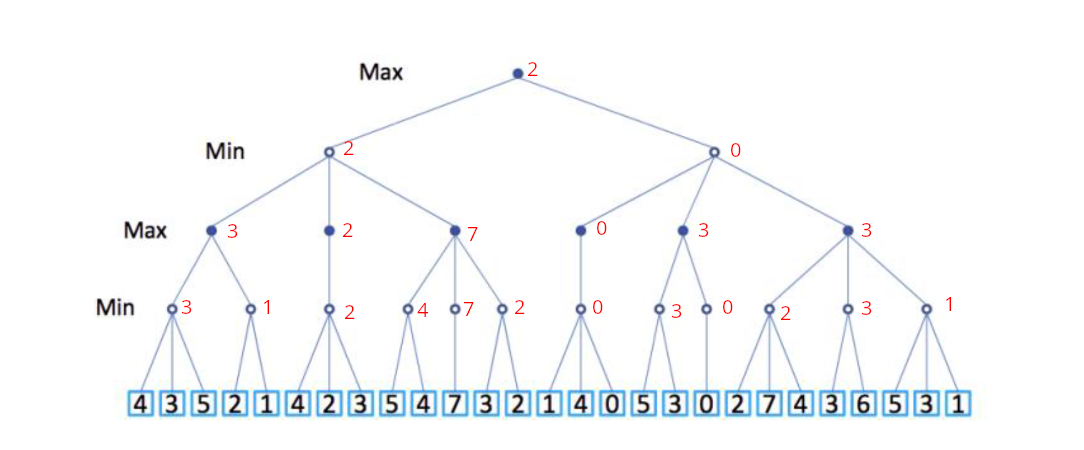
\includegraphics[scale=1.5]{zum-3-1.png}
    \caption{Průběh MiniMax}
    \label{fig:enter-label}
\end{figure}

\begin{figure}[h!]
    \centering
    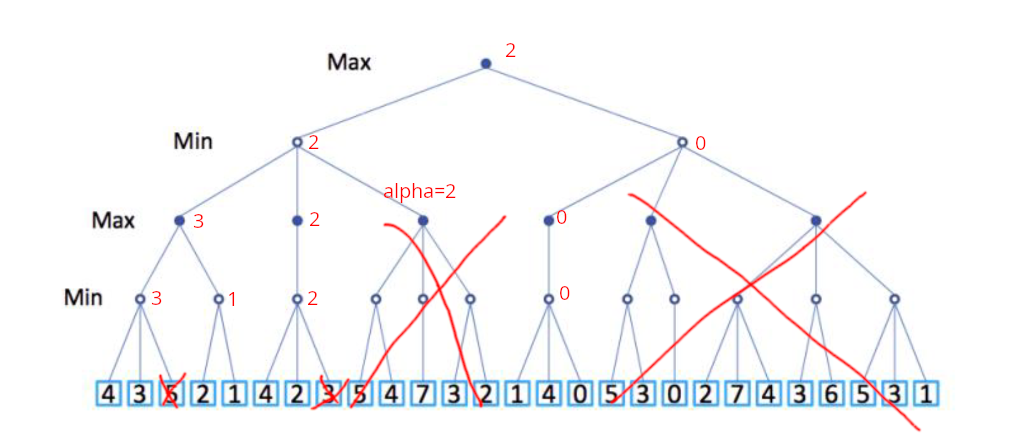
\includegraphics[scale=1.5]{zum-3-2.png}
    \caption{Průběh MiniMax s $\alpha\beta$ prořezaváním}
    \label{fig:enter-label}
\end{figure}

\end{document}
